\section{Результати}

Тестування відбувалося на машині із процесором Intel Core i7-8550U 1.99GHz під 64-бітною версією операційної системи Windows.

\begin{figure}[H]
    \centering
    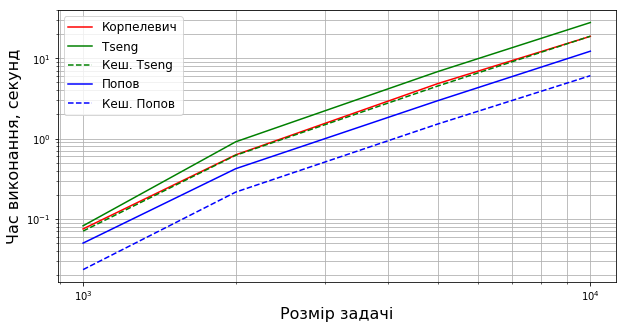
\includegraphics[width=.75\textwidth]{img/1/time.png}
\end{figure}

І справді, бачимо що алгоритм Корпелевич і кешований алгоритм Tseng'a справді показують майже однакові результати, а також обидві некешовані версії програють кешованим. Та сама інформація у табличці, для зручності:

\begin{table}[H]
	\centering
	\begin{tabular}{|c||c|c|c|c|}\hline
		Розмір задачі & 1000 & 2000 & 5000 & 10000 \\ \hline \hline
		Корпелевич & 0.11 & 0.65 & 4.95 & 19.31 \\ \hline
		Tseng & 0.10 & 0.98 & 7.13 & 26.82 \\ \hline
		Кеш. Tseng & 0.07 & 0.71 & 4.49 & 17.98 \\ \hline
		Попов & 0.08 & 0.50 & 2.98 & 12.18 \\ \hline
		Кеш. Попов & 0.03 & 0.26 & 1.52 & 6.16 \\ \hline
	\end{tabular}
	\caption{Час виконання, секунд}
\end{table}


\begin{table}[H]
	\centering
	\begin{tabular}{|c||c|c|c|c|}\hline
		Розмір задачі & 1000 & 2000 & 5000 & 10000 \\ \hline \hline
		Корпелевич & 132 & 137 & 144 & 148 \\ \hline
		Tseng & 132 & 137 & 144 & 148 \\ \hline
		Попов & 89 & 92 & 96 & 99 \\ \hline
		Маліцький Tam & 91 & 94 & 98 & 101 \\ \hline
	\end{tabular}
	\caption{Число ітерацій}
\end{table}


\begin{remark}
    Наша реалізація приблизно у 50 разів швидша за результати наведені у статті \href{https://arxiv.org/abs/1502.04968v1}{[Yura Malitsky, 2015]}. Зміна мови програмування і краща машина приблизно у рівниій мірі відповідають за прискорення.
\end{remark}

\section{Розріджені матриці}

Нескладно помітити, що матриця $A$ дуже розріджена, що наводить на ідею скористатися модулем scipy.sparse для ефективної роботи з розрідженими матрицями. Це дозволить нам розв'язувати задачу для значно більших $m$.

\begin{figure}[H]
    \centering
    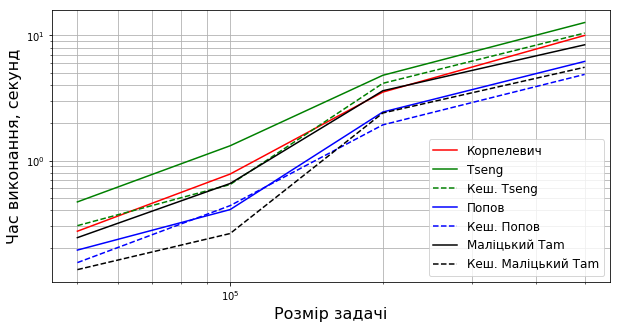
\includegraphics[width=.75\textwidth]{img/1/sparse/time.png}
\end{figure}

Та сама інформація у табличці, для зручності:

\begin{table}[H]
	\centering
	\begin{tabular}{|c||c|c|c|c|}\hline
		Розмір задачі & 50000 & 100000 & 200000 & 500000 \\ \hline \hline
		Корпелевич & 0.06 & 0.24 & 2.04 & 3.56 \\ \hline
		Tseng & 0.08 & 0.38 & 1.78 & 5.56 \\ \hline
		Кеш. Tseng & 0.07 & 0.21 & 1.35 & 5.22 \\ \hline
		Попов & 0.04 & 0.10 & 1.03 & 2.82 \\ \hline
		Кеш. Попов & 0.03 & 0.13 & 1.13 & 2.73 \\ \hline
	\end{tabular}
	\caption{Час виконання, секунд}
\end{table}


\begin{table}[H]
	\centering
	\begin{tabular}{|c||c|c|c|c|}\hline
		Розмір задачі & 50000 & 100000 & 200000 & 500000 \\ \hline \hline
		Корпелевич & 255 & 260 & 265 & 271 \\ \hline
		Tseng & 255 & 260 & 265 & 271 \\ \hline
		Кеш. Tseng & 255 & 260 & 265 & 271 \\ \hline
		Попов & 168 & 171 & 174 & 178 \\ \hline
		Кеш. Попов & 168 & 171 & 174 & 178 \\ \hline
		Маліцький Tam & 170 & 173 & 176 & 180 \\ \hline
		Кеш. Маліцький Tam & 170 & 173 & 176 & 180 \\ \hline
	\end{tabular}
	\caption{Число ітерацій}
\end{table}


\begin{remark}
    Тут перевага кешування вже не така очевидна, адже ми значно здешевили обчислення оператора $A$, хоча все ще присутня.
\end{remark}
